% Appendix 7: Reverse Perspective and Lobachevsky Geometry
% Source pages: 270–274

\chapter{Reverse Perspective and Lobachevsky Geometry}

\srcpage{270}

As is well known, objective external space (meaning the objects with which the artist
deals) may be considered Euclidean.  In the process of transforming this space into
perceptual space it undergoes substantial deformations, so that its geometry is not obvious.

In 1947, Luneburg showed that in its properties perceptual space may be considered a
space of Lobachevsky.\footnote{A brief account of Luneburg's work and bibliography: see
  S.~Koch (Ed.).\ \emph{Psychology: A Study of a Science}, vol.\,I\@. New York, 1959.}
Luneburg based this conclusion on the well-known experiments of
Blumenfeld,\footnote{W.~Blumenfeld.  Untersuchungen \"uber die scheinbare Gr\"o\ss e im
  Sehraume.---\emph{Z.~Psychol.~Physiol.~Sinnesorgane}, 1913, 65, S.\,241.}
in which it was established that if a subject observing two rows of points on a horizontal
plane is asked first to arrange the points so that the rows appear \emph{parallel}, and
then to arrange them so that the distance between them appears \emph{constant}, the subject
places the points differently in the two experiments.  In Euclidean space, parallel lines
and everywhere-equidistant lines should coincide, so the discrepancy recorded by Blumenfeld
may be interpreted as indicating that perceptual space is non-Euclidean.  Both the
Blumenfeld experiments and a series of special experiments carried out to confirm Luneburg's
theory showed that for sections of a horizontal plane in the immediate vicinity of the
observer, the properties of perceptual space can indeed be described as properties of
Lobachevsky space.

In accordance with the experimental limitations existing at the present time, we consider
only the problem of transforming by the human perceptual system the retinal image of a
section of a horizontal plane of comparatively small extent.

\srcpage{271}

\begin{figure}[H]
    \centering
    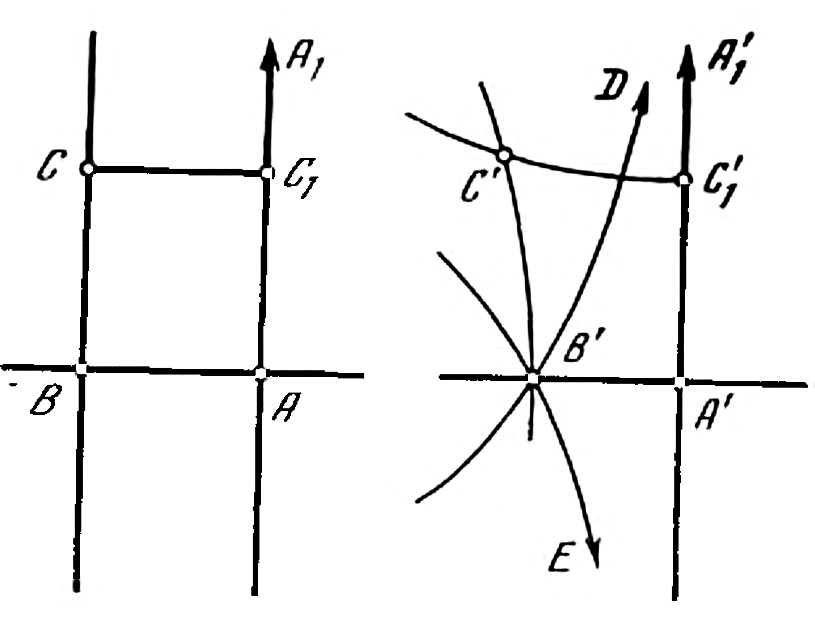
\includegraphics[width=0.55\linewidth]{figures/f7.1.png}
\end{figure}
\figblock{7.1}{Diagram (view from above) of the experiment in objective space (right
  half) and perceptual space (left half).  Objective rectangle $ABCC_1$ (with a right
  angle at each vertex) corresponds to Lambert quadrilateral $A'B'C'C_1'$ (with right
  angles at $A'$, $B'$, $C_1'$ only) in perceptual Lobachevsky space.  The far side
  $C'C_1' = k$ exceeds the near side $A'B' = a$, giving reverse perspective.}

Let the observer stand at point~$A$ in objective space on a flat horizontal patch, looking
in direction~$AA_1$ (Fig.\,7.1).  Draw $AB$ perpendicular to $AA_1$, directed along the
observer's shoulder line.  Through~$B$ draw $BC$ parallel to~$AA_1$ (in Euclidean space
this can be done in a unique way).  Drop a perpendicular from~$C$ to~$AA_1$; the result is
rectangle~$ABCC_1$.

Consider the configuration of this rectangle in perceptual space, making the natural
assumption that straight lines of objective space correspond to straight lines of perceptual
space.\footnote{This assumption, which underlies the subsequent reasoning, amounts to
  supposing that the line joining two points of perceptual space by the shortest path is
  the image of the line joining the corresponding points of objective space by the shortest
  path.  Such an assumption is sufficiently natural and biologically reasonable, since
  correct assessment of shortest distances is essential from a biological standpoint, and
  both humans and animals are guided in their behaviour by the images arising in perceptual
  space.}
Let point~$A$ correspond to point~$A'$ in perceptual space, and line~$AA_1$ to
line~$A'A_1'$.  By the symmetry that must hold between the left and right half-planes in
the observer's consciousness, line~$A'A_1'$ cannot curve in perceptual space.  Lay off
from~$A'$ the segment~$A'B'$, perpendicular to~$A'A_1'$, corresponding to segment~$AB$ of
objective space.  The line $A'B'$ is also straight in the observer's mind, since he must
perceive the upper and lower half-planes as symmetric.  Continue the construction as in
objective space.  If one starts from the experimental fact that perceptual space is a
Lobachevsky space, then through point~$B'$ one can draw \emph{two} parallels to~$A'A_1'$,
namely~$B'D$ and~$B'E$, and in addition all the infinitely many Lobachevsky lines lying
between $B'D$ and $B'E$ will also never intersect~$A'A_1'$.  Instead of the unique
line~$BC$ that does not meet~$AA_1$, the construction has thus produced infinitely many.

\srcpage{272}

To select from this family the unique Lobachevsky line corresponding to $BC$ in objective
space, one can use neither the notion of parallelism (non-intersection with~$A'A_1'$, a
property shared by the whole family) nor the notion of equidistance (no member of the
family is equidistant from~$A'A_1'$ in the Lobachevsky metric).\footnote{Were one to
  construct the line through~$B'$ equidistant from~$A'A_1'$, it would, as is well known,
  not be a straight line in Lobachevsky geometry.}  The way out is to use the mirror
symmetry of the upper and lower half-planes in the diagram of objective space.

Indeed, $AB$ may be regarded as an axis of symmetry.  Requiring the Lobachevsky line
through~$B'$ to be symmetric with respect to~$A'B'$ singles out from the family a unique
line~$B'C'$, which by that symmetry property must intersect~$A'B'$ at right angles.  Take
on~$B'C'$ the point~$C'$ corresponding to~$C$ in objective space, and drop a perpendicular
from~$C'$ to~$A'A_1'$.  The resulting quadrilateral~$A'B'C'C_1'$ corresponds to
rectangle~$ABCC_1$ of objective space.\footnote{The correspondence obtained is not only
  formally mathematical; it is conditioned in particular by the fact that in the method of
  construction adopted, the possibilities of human psychology are taken into account.
  Indeed, the right angle at vertex~$A'$ can be constructed because that vertex corresponds
  to the point where the observer stands, and the right angles at~$B'$ and~$C_1'$ can be
  constructed because foreshortening does not distort the visible magnitudes of the angles
  at~$B$ and~$C_1$.}
The quadrilateral~$A'B'C'C_1'$ has three right angles---at~$B'$ by symmetry, and at~$A'$
and~$C_1'$ by construction.  Such a quadrilateral is sometimes called a \emph{Lambert
quadrilateral}.  For a Lambert quadrilateral there is a well-known relation connecting the
sides $a$ and $b$ enclosed between the right angles with the side~$k$ opposite to~$a$
(in Fig.\,7.1: $a = A'B'$, \, $b = A'C_1'$, \, $h = C'C_1'$):
\begin{equation}
  \cos\Pi(a) = \cos\Pi(h)\,\sin\Pi(b),  \tag{7.1}
\end{equation}
where $\Pi(x)$ is the Lobachevsky function (angle of parallelism), defined by
\begin{equation}
  \Pi(x) = 2\arctan e^{-x/R}.  \tag{7.2}
\end{equation}
Here $R$ is the curvature radius of the Lobachevsky space.

\srcpage{273}

From relation~(7.1), noting that $\Pi(x) < \pi/2$ for $x > 0$, it follows that
$\sin\Pi(b) < 1$, and consequently $\cos\Pi(h) > \cos\Pi(a)$.  Since $\Pi(x)$ is a
decreasing function, this gives
\[
  k > a,
\]
i.e.\ in perceptual space the far side of the quadrilateral exceeds the near side.
\emph{This is the reverse perspective.}

Turning to everyday human experience, several facts suggest that the Lobachevskian
properties of perceptual space are characteristic only of a comparatively small region
surrounding the observer, while more distant regions must be described by Riemannian
geometry of positive curvature.  This is indicated by the familiar fact of spatial visual
perception---all objectively parallel lines are perceived as converging to a point on the
horizon.  Since everyday experience leads one to suppose that distant regions of perceptual
space have positive curvature, while the experiments connected with Luneburg's theory show
that the immediately surrounding perceptual space has negative curvature, one may conjecture
that the curvature of perceptual space is \emph{variable}.  The corresponding Riemannian
space model must therefore have some positive curvature at large distances from the
observer, gradually diminishing as one approaches him, and becoming negative in his
immediate vicinity (under binocular vision).

Without aiming to specify here the only-sketched properties of the Riemannian space of
variable curvature, we note only that the geometry of perceptual space is in fact even more
complex.  The closest analogy of perceptual space is \emph{Einstein space}.  In Einstein's
general theory of relativity, space has variable curvature depending on the masses
contained in it.  Recall, however, that at the end of Chapter~III, when discussing
Ill.\,26, it was shown that the geometric properties of perceptual space depend on the
objects depicted in it.  In this connection, if one speaks of an analogy between Einstein
space and perceptual space, then in the latter, \emph{a priori} information plays a role
analogous to that of mass in general relativity: just as an increase of mass in some region
of physical space increases its curvature, an increase of a priori information about the
objects in some region of perceptual space increases its deformation.

\srcpage{274}

All the questions touched upon here are still entirely undeveloped and can be advanced only
through the mathematical processing and interpretation of a series of carefully designed
experiments.
